\begin{itemize}
	\item To fill the nationally recognized research gap in understanding potential Earth system feedbacks of SAI on ecosystems, regional atmospheric circulation, and biogeochemical cycles, we will conduct a series of increasingly complex geoengineering simulations, using \textbf{DOE's Energy Exascale Earth System Model (E3SM)}.

	\item \textbf{These simulations will mimic the effects of CDR, SAI, and CDR plus SAI in combination.}

	\item We will start with the well-defined SSP5-3.4-OS mid-range overshoot CO$_2$ trajectory from CMIP6, which prescribes a drawdown of atmospheric CO$_2$ due to CDR, large reductions in emissions, or both.

	\item In that scenario, global surface temperatures rise by $>$2.5$^\circ$C around 2040, \textbf{well above the 2$^\circ$C threshold that may induce irreversible impacts}.

	\item A second set of simulations would introduce SAI to simultaneously cool the surface, or \textbf{``shave'' the temperature peak}, until drawdown is sufficient to assure $<$2$^\circ$ warming at any time as illustrated in Figure~\ref{fig:peak_shaving}B.
\end{itemize}

\vskip0.25in

\begin{figure}
	\begin{center}
		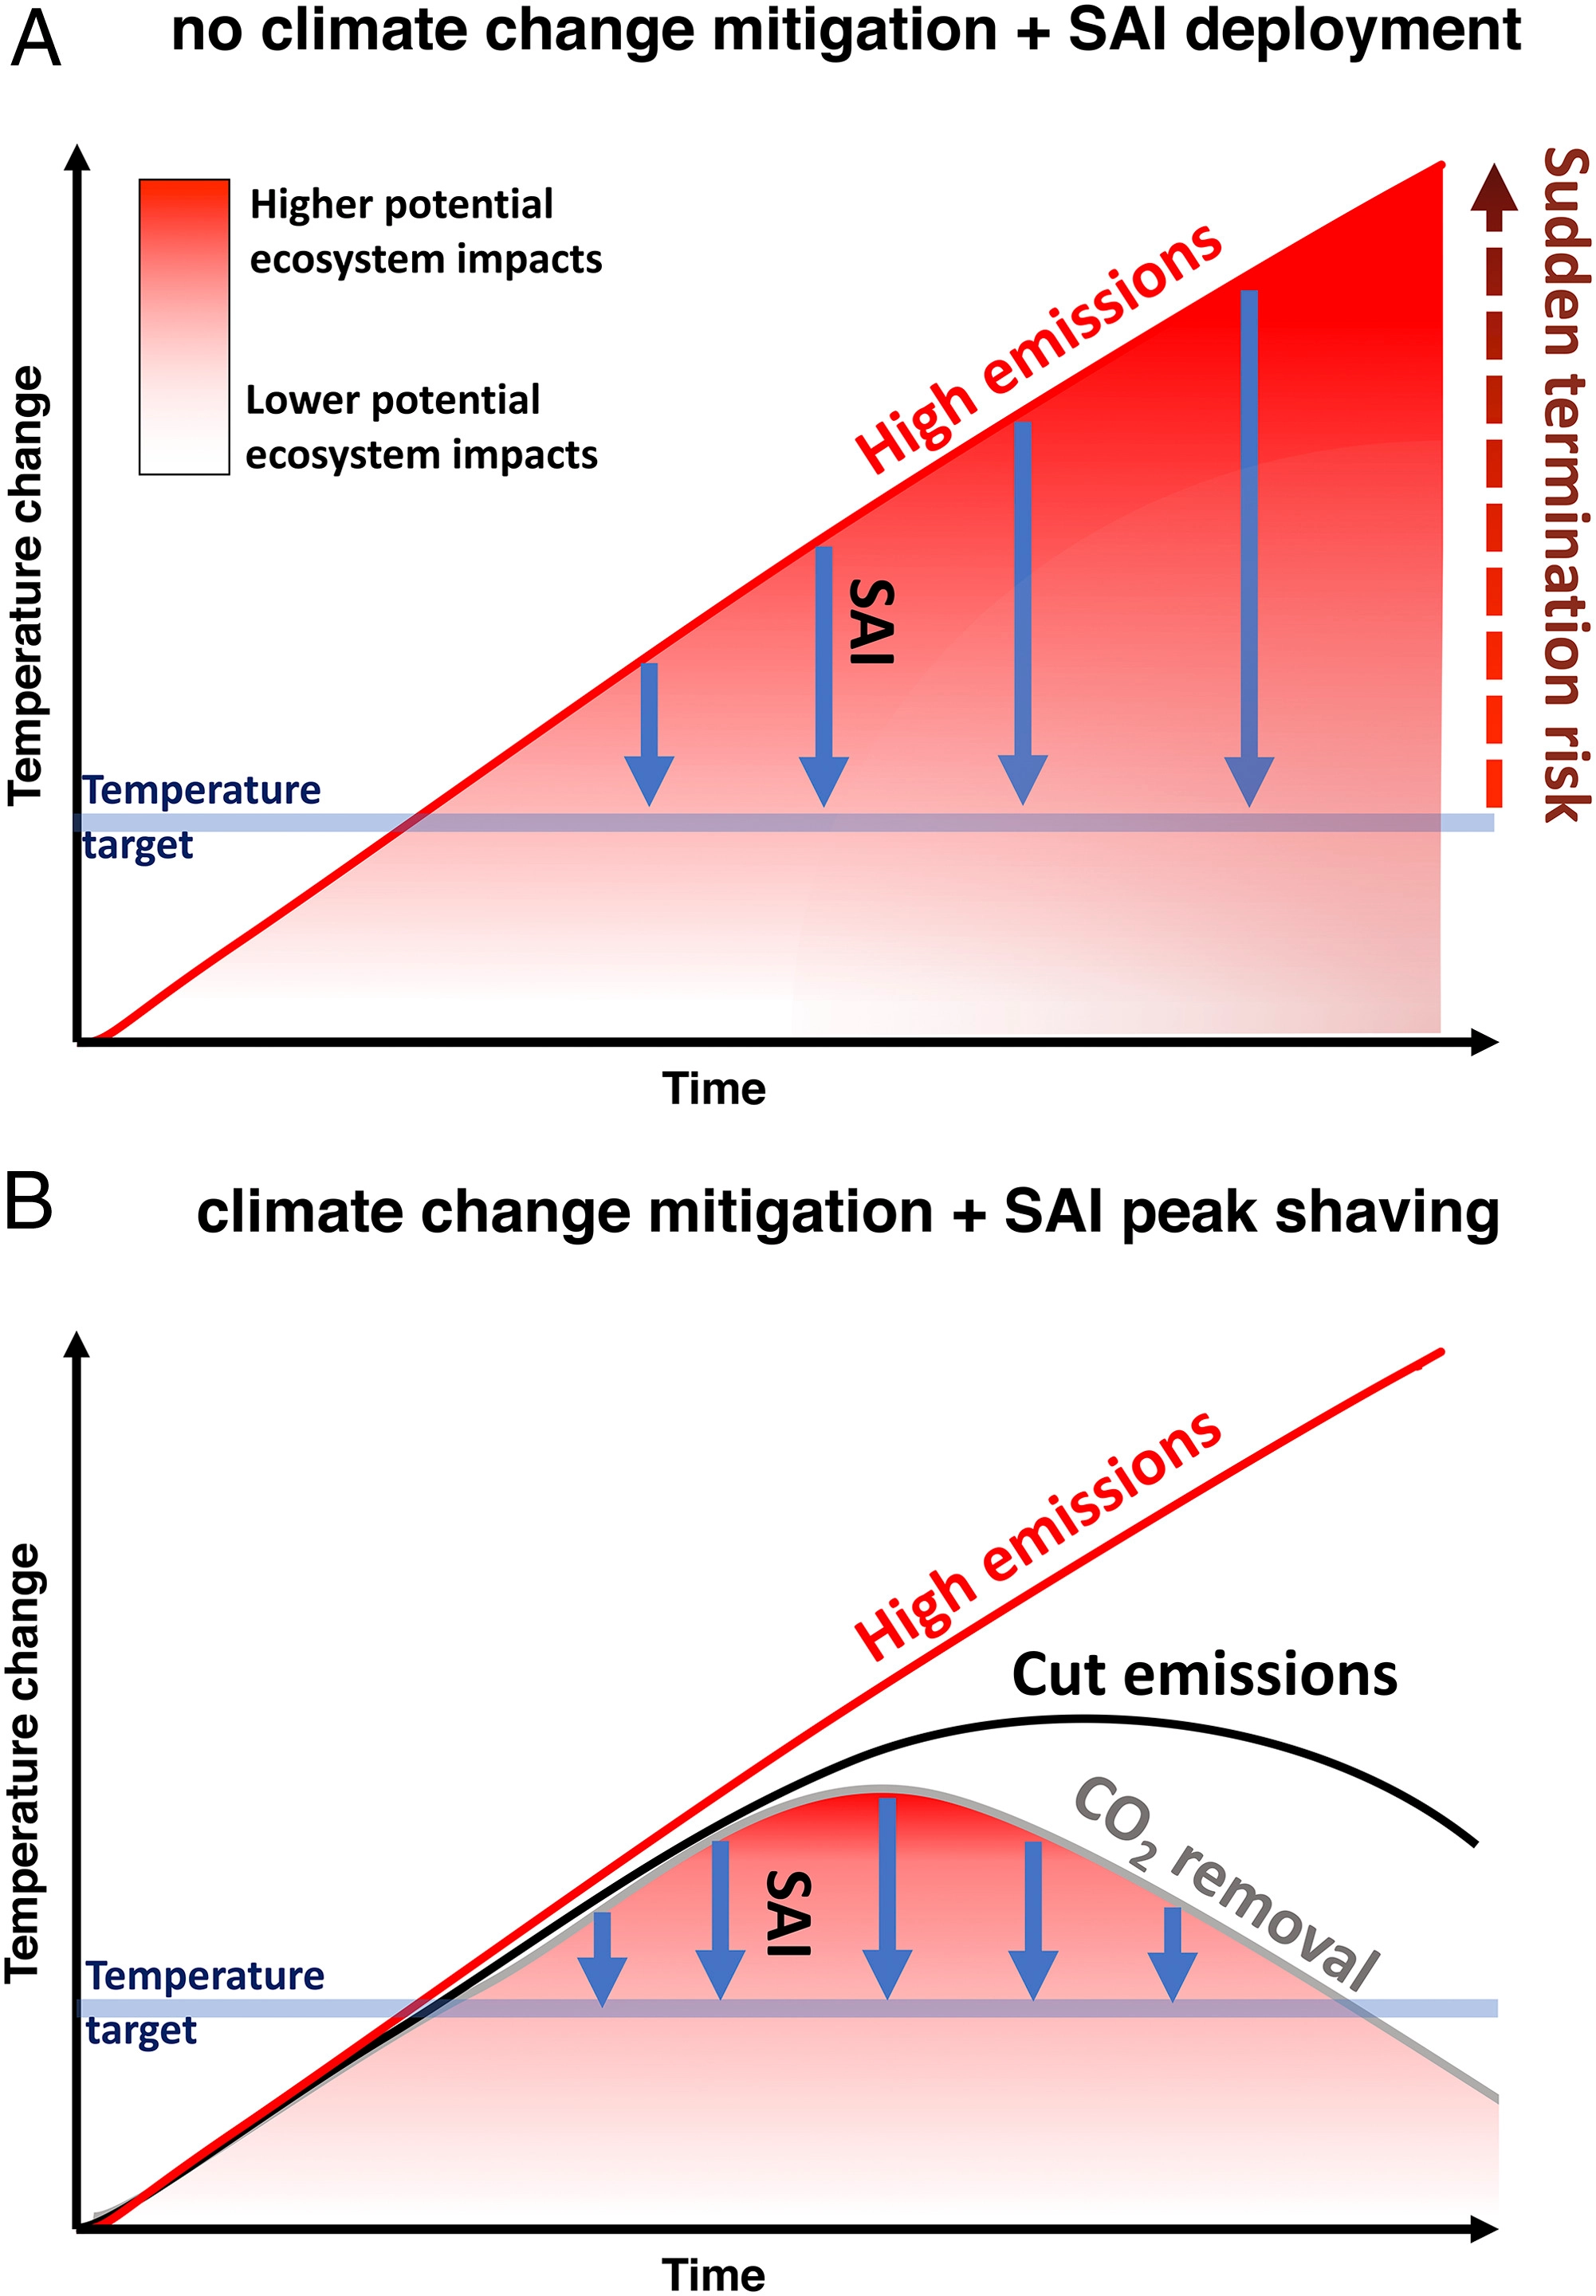
\includegraphics[trim=0cm 52.0cm 0cm 0cm,clip=true,width=0.48\columnwidth]{figures/pnas_fig2.png} \hfill
		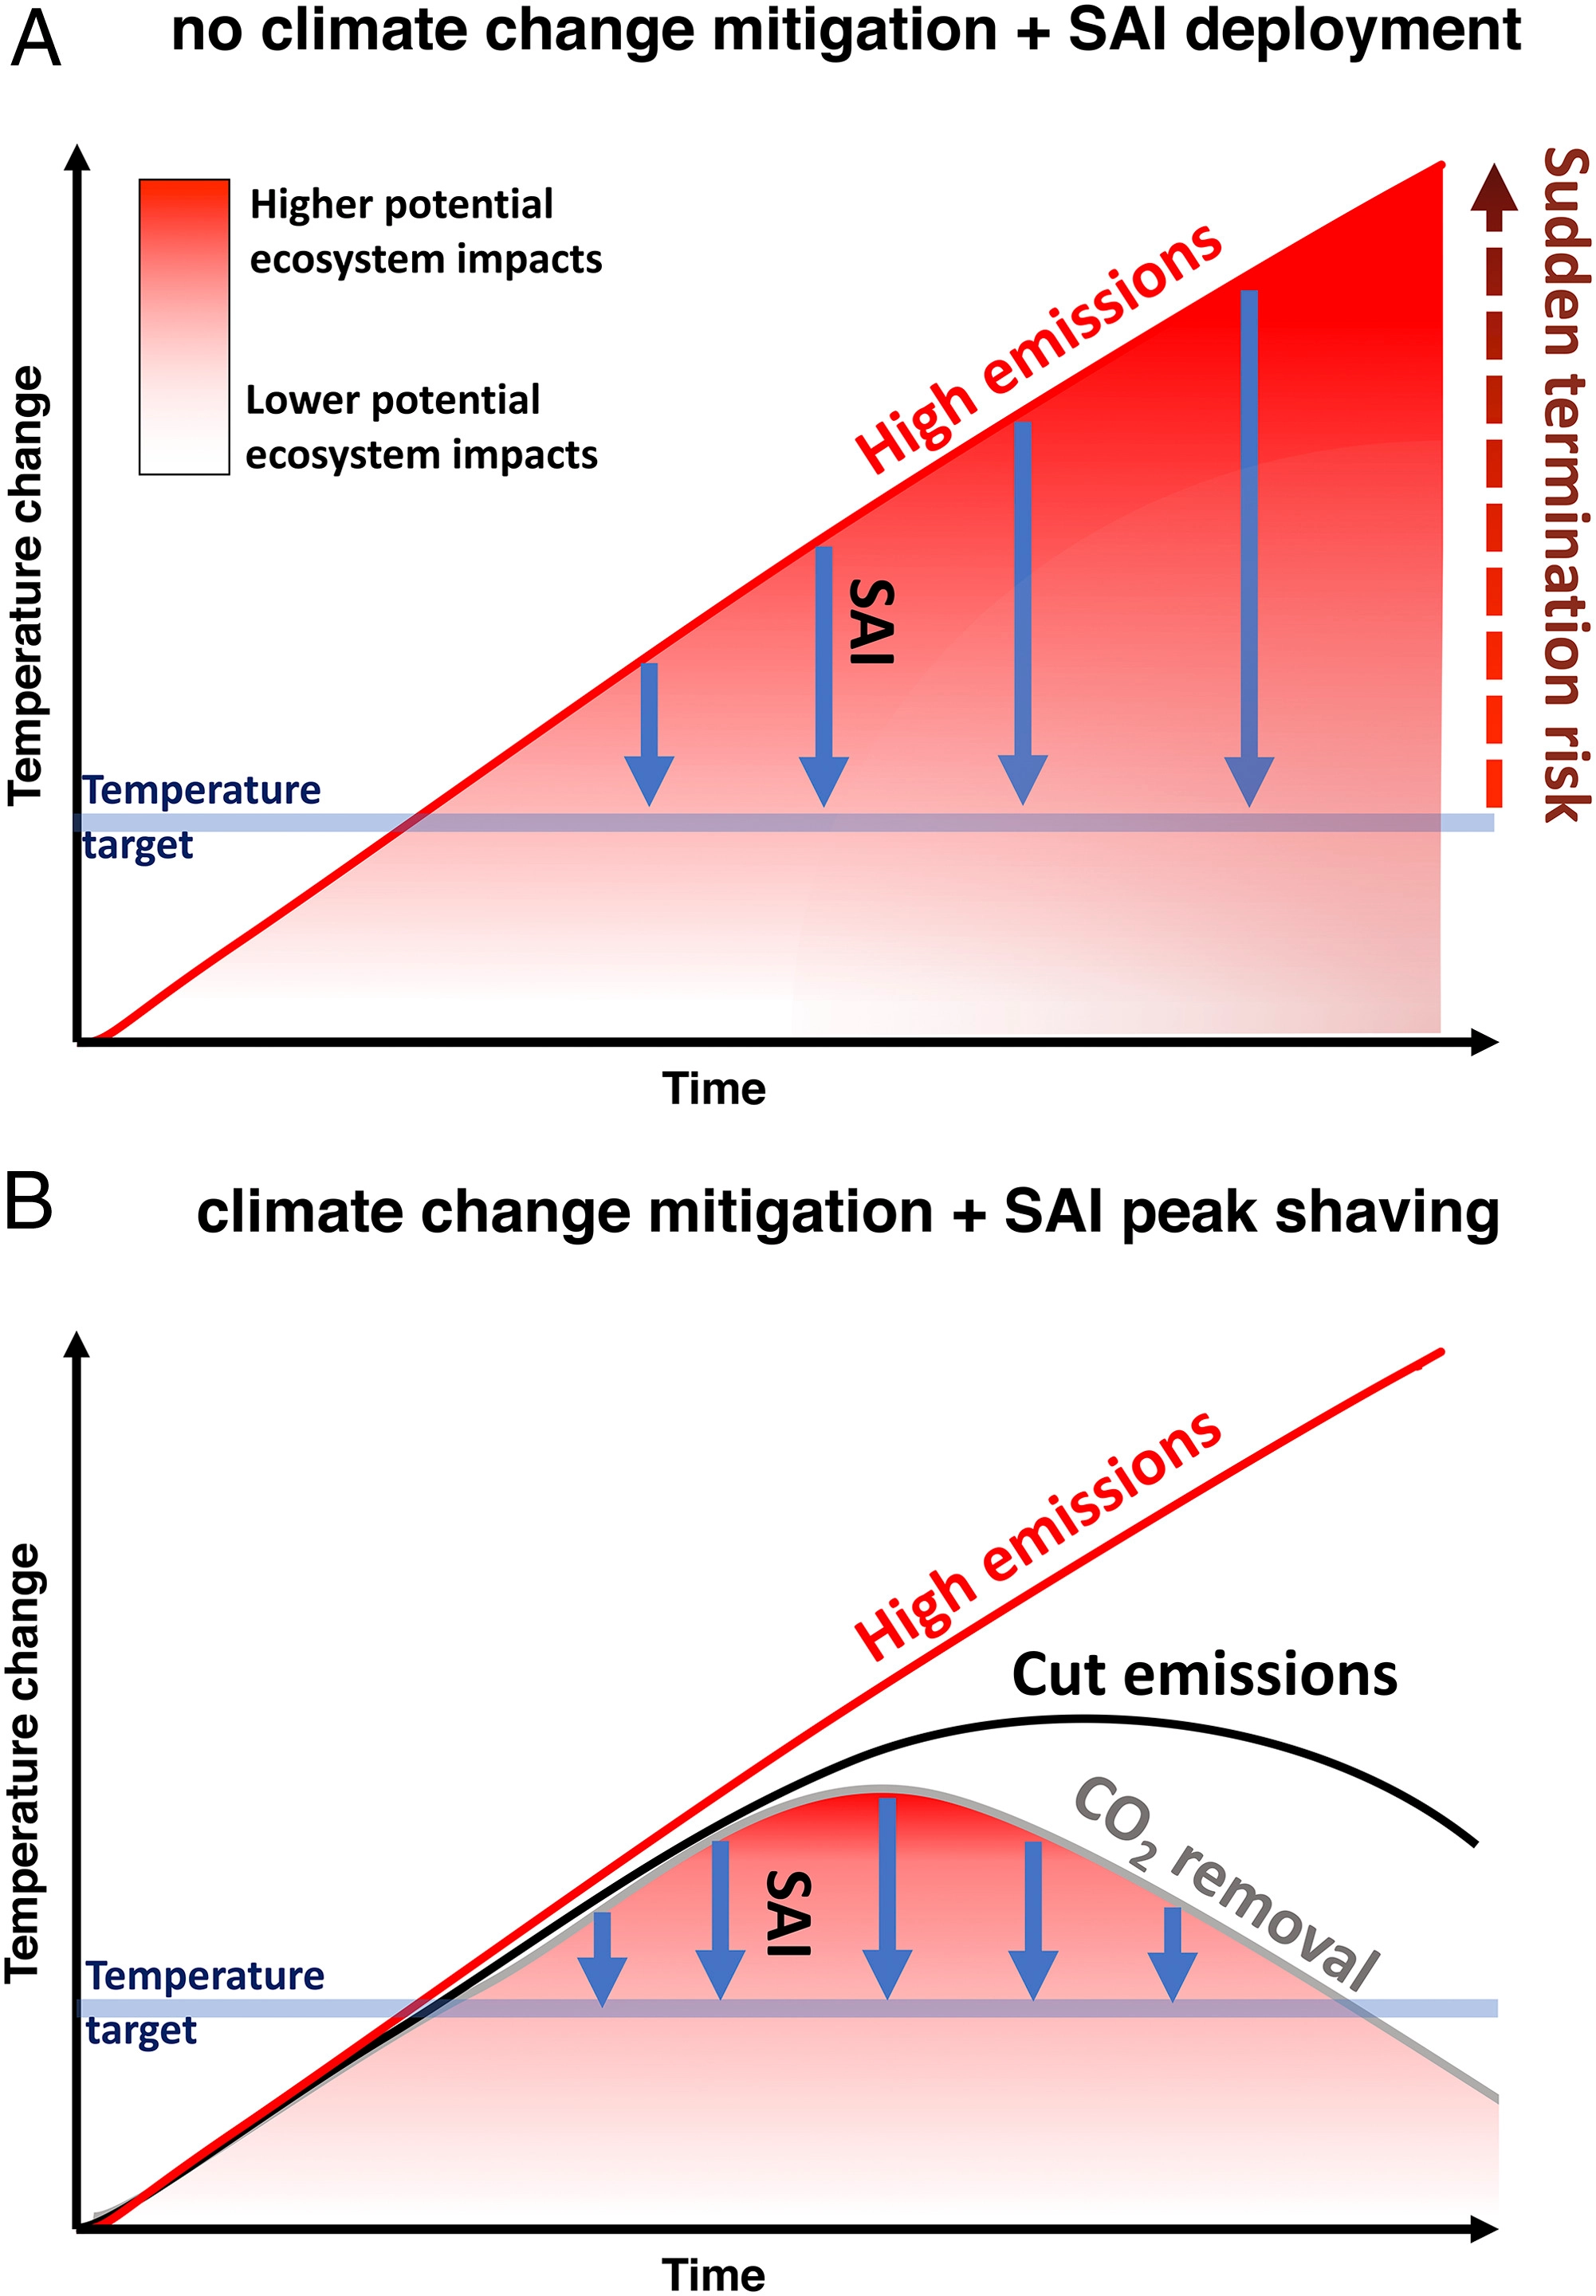
\includegraphics[trim=0cm 0cm 0cm 51.89cm,clip=true,width=0.48\columnwidth]{figures/pnas_fig2.png}
	\end{center}
	\caption{Potential temperature change over time for two different SAI scenarios. (A) In a future with no climate change mitigation and with SAI deployment, high emissions result in rising temperatures (red line). Increasing amounts of SAI would have to be deployed to reduce temperature (blue arrows) to a specific temperature target (blue line). The risk of sudden SAI termination also increases (red arrow). (B) In a future with climate change mitigation and SAI ``peak shaving,'' temperature changes are first reduced by a combination of emissions reductions (black line) and CDR (CO$_2$ removal, gray line), then further reduced by SAI (blue arrows).
		%The red shaded areas below the two curves indicate the potential overall risk for ecological systems from increased temperature and SAI deployment; carbon emissions alone would not create the same degree of risk reduction as shown in B.
		%We note that SAI is not akin to a global thermostat that would only control global temperatures to remediate GHG-induced warming. GHGs add energy to the system at the surface and throughout the atmosphere, whereas reducing sunlight with SAI only changes the energy balance at Earth's surface. Furthermore, GHGs operate 24 h a day and all year long, whereas reducing sunlight primarily has a direct impact during the daytime and more so in summer than winter.
		Adopted from Zarnetske et al. (2021).
		% https://www.pnas.org/doi/10.1073/pnas.1921854118
	}\label{fig:peak_shaving}
\end{figure}

\vskip0.25in

\begin{figure}
	\begin{center}
		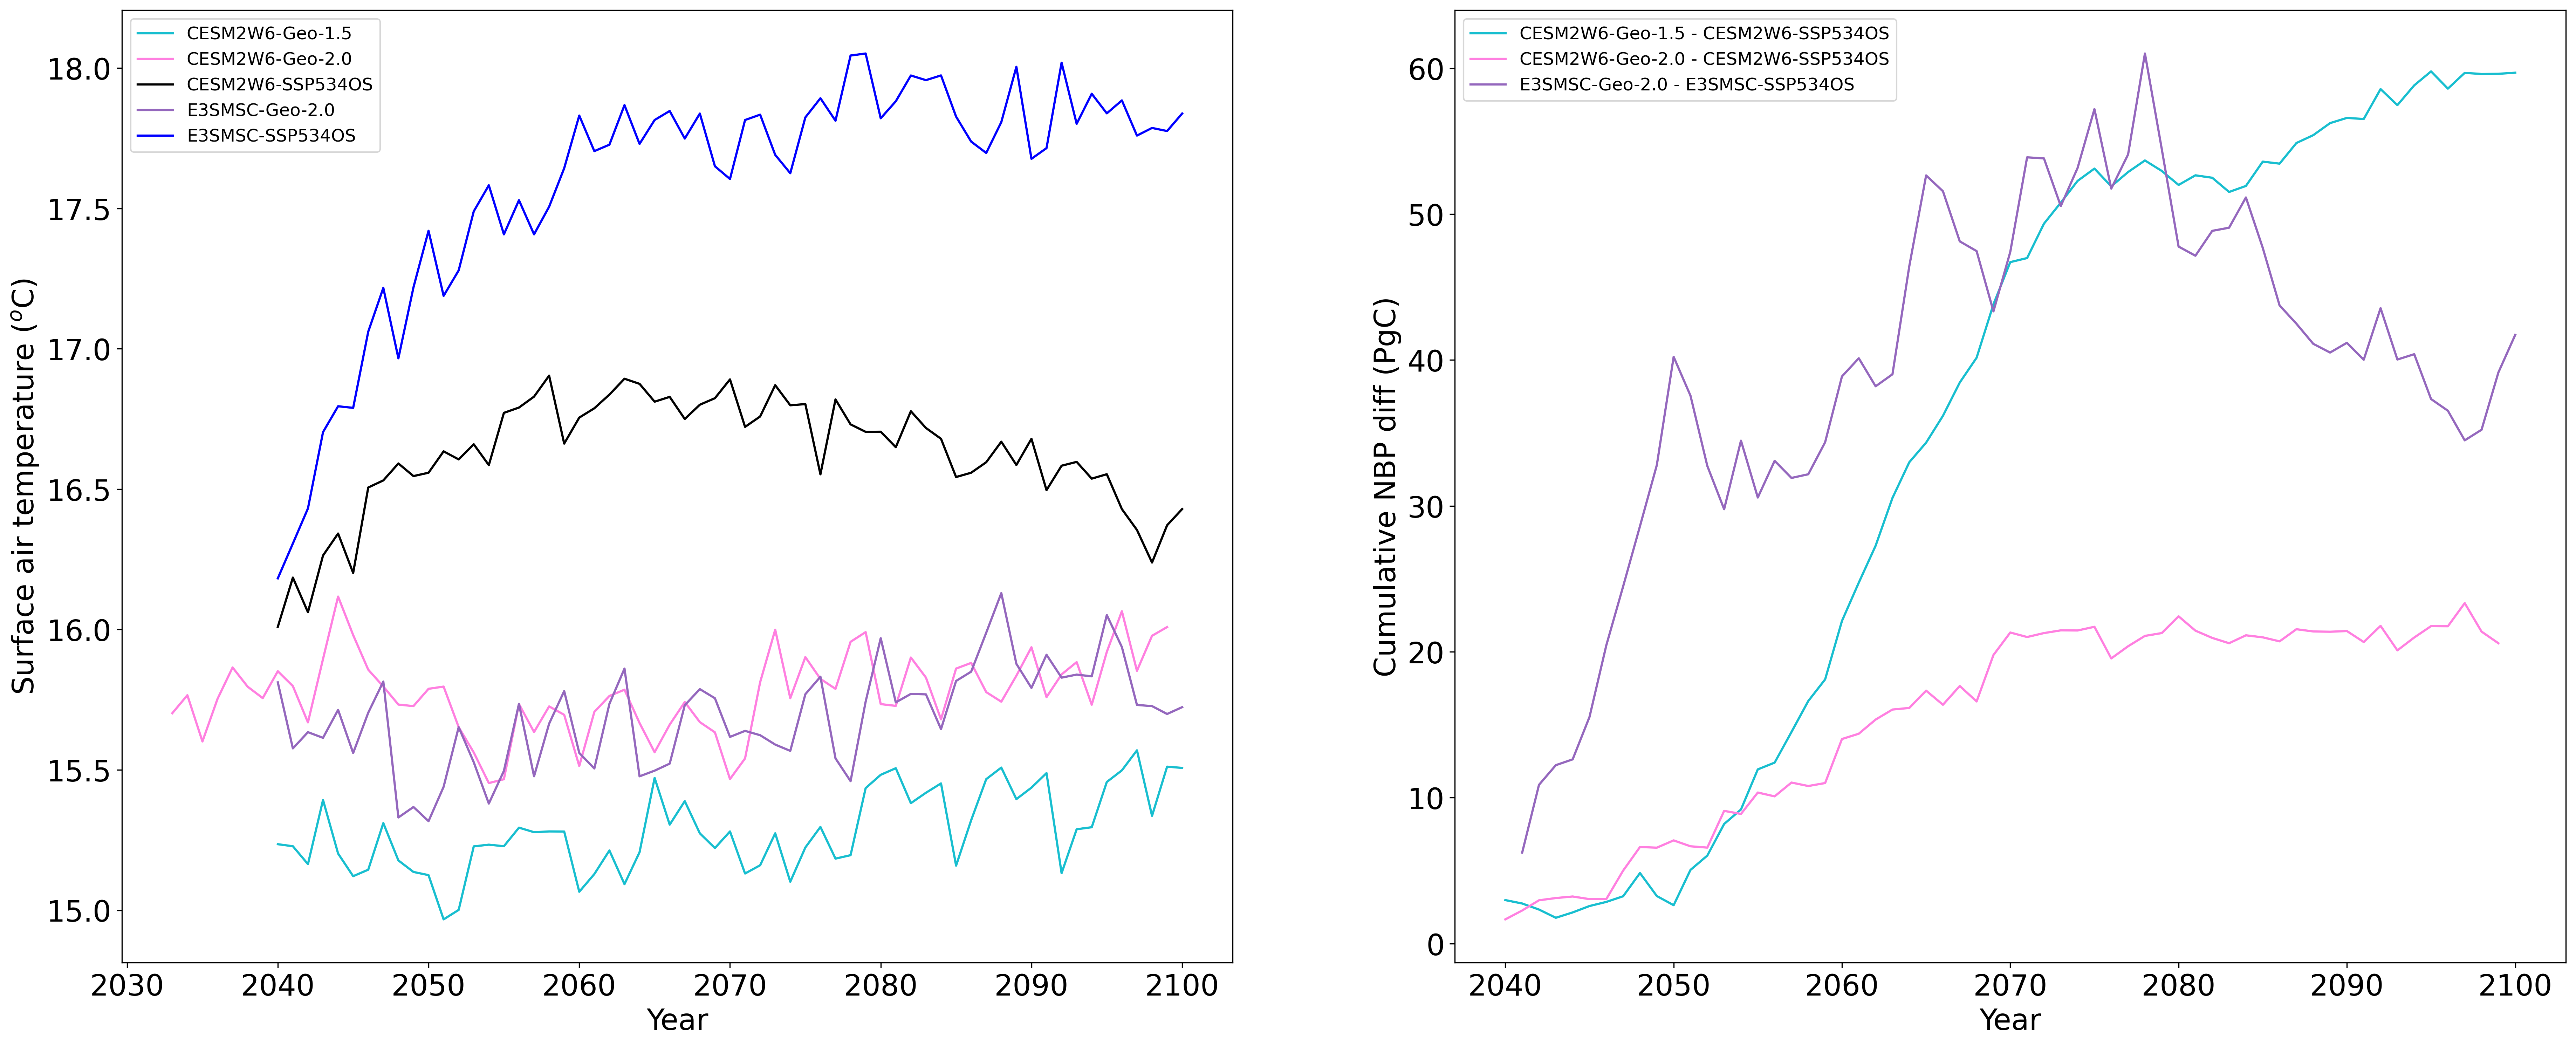
\includegraphics[width=\columnwidth]{figures/e3sm_geo_global_ts_tas_nbp.png}
	\end{center}
	\caption{Such ``peak shaving'' simulations have been performed with the Community Earth System Model version 2 (CESM2) and E3SM. In all simulations, the SSP5-3.4-OS scenario was used, first without SAI then with SAI. CESM2 was used to simulate both 1.5\,$^\circ$ and 2.0\,$^\circ$ temperature targets, and E3SM has so far been used to simulate a 2.0$^\circ$ temperature target. (Left) Surface temperature for the baseline SSP5-3.4-OS simulations and a single ensemble member of 1.5\,$^\circ$ and 2.0\,$^\circ$ simulations from CESM2 and the 2.0\,$^\circ$ simulation from E3SM. (Right) The cumulative difference in land carbon storage for the three SAI scenarios represented in the panel at left. In all cases, SAI induced a stronger land carbon sink. By the year 2100, the 1.5\,$^\circ$ simulation from CESM2 had the largest increase in land carbon storage, the CESM2 2.0\,$^\circ$ simulation has the smallest increase, and the E3SM 2.0\,$^\circ$ simulation ended up in between the other two.}\label{fig:e3sm_tas_nbp}
\end{figure}

\vskip0.25in

\begin{figure}
	\begin{center}
		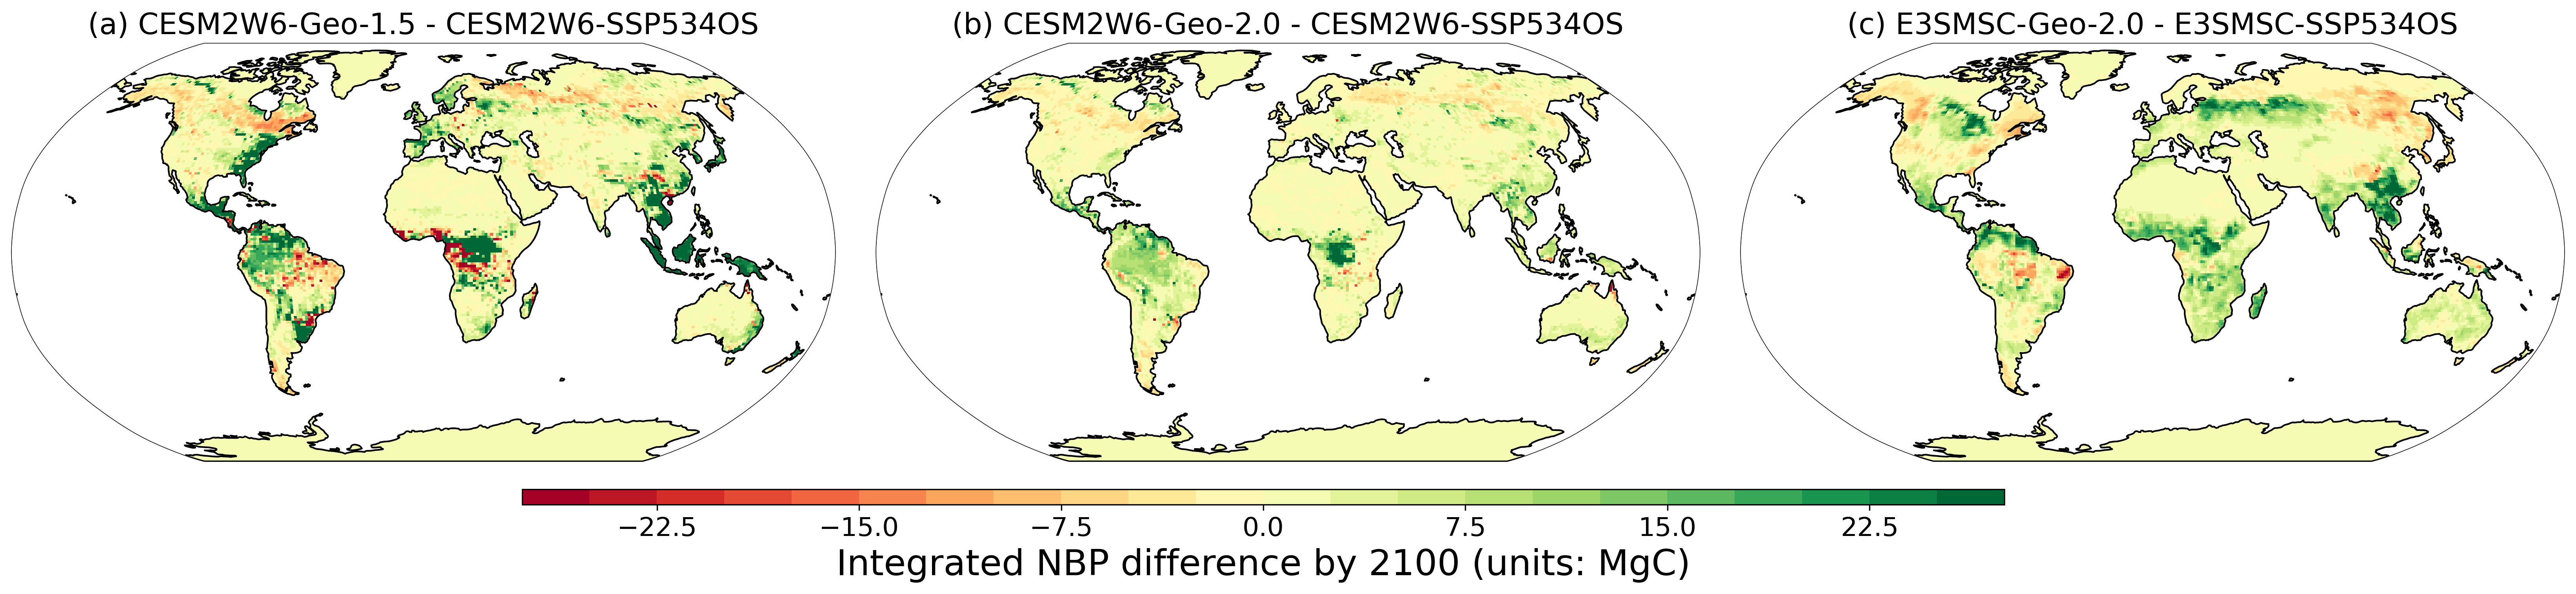
\includegraphics[width=\columnwidth]{figures/e3sm_geo_nbp_map.png}
	\end{center}
	\caption{The spatial distribution of the cumulative change in land carbon storage varied across the three simulations. The global spatially integrated trajectories of these integrated land carbon storage changes is shown in the right-hand panel in Figure~\ref{fig:e3sm_tas_nbp}.}\label{fig:e3sm_nbp_map}
\end{figure}

\begin{itemize}
	\item \textbf{These and other scenario simulations must be performed and analyzed to determine the effects of reduced radiative forcing despite increasing atmospheric CO$_2$ levels on Earth's climate, regional atmospheric dynamics and aerosol-cloud interactions, and terrestrial and marine carbon sink strengths.}

	\item \textbf{This research will better characterize and reduce scientific and societal uncertainties concerning the benefits and risks of solar geoengineering deployment, so that informed decisions can be made in the future about possible implementation.}

\end{itemize}


